\let\negmedspace\undefined
\let\negthickspace\undefined
\documentclass[journal]{IEEEtran}
\usepackage[a5paper, margin=10mm, onecolumn]{geometry}
%\usepackage{lmodern} % Ensure lmodern is loaded for pdflatex
\usepackage{tfrupee} % Include tfrupee package

\setlength{\headheight}{1cm} % Set the height of the header box
\setlength{\headsep}{0mm}     % Set the distance between the header box and the top of the text

\usepackage{gvv-book}
\usepackage{gvv}
\usepackage{cite}
\usepackage{amsmath,amssymb,amsfonts,amsthm}
\usepackage{algorithmic}
\usepackage{graphicx}
\usepackage{textcomp}
\usepackage{xcolor}
\usepackage{txfonts}
\usepackage{listings}
\usepackage{enumitem}
\usepackage{mathtools}
\usepackage{gensymb}
\usepackage{comment}
\usepackage[breaklinks=true]{hyperref}
\usepackage{tkz-euclide} 
\usepackage{listings}
% \usepackage{gvv}                                        
\def\inputGnumericTable{}                                 
\usepackage[latin1]{inputenc}                                
\usepackage{color}                                            
\usepackage{array}                                            
\usepackage{longtable}                                       
\usepackage{calc}                                             
\usepackage{multirow}                                         
\usepackage{hhline}                                           
\usepackage{ifthen}                                           
\usepackage{lscape}
\begin{document}

\bibliographystyle{IEEEtran}
\vspace{3cm}

\title{2.10.30}
\author{EE25BTECH11001 - Aarush Dilawri}
% \maketitle
% \newpage
% \bigskip
{\let\newpage\relax\maketitle}

\renewcommand{\thefigure}{\theenumi}
\renewcommand{\thetable}{\theenumi}
\setlength{\intextsep}{10pt} % Space between text and floats
\textbf{Question}:\\
The points with position vectors $60\vec{i} + 3\vec{j}$, $40\vec{i} - 6\vec{j}$, $a\vec{i} - 52\vec{j}$ are collinear if\\
\begin{multicols}{2}
\begin{enumerate}[label=(\alph*)]
    \item  a = -40
    \item  a = 40
    \item  a = 20
    \item  None of these
\end{enumerate}
\end{multicols}
\textbf{Solution}:\\
We have position vectors
\begin{align}
\vec{A} &= \myvec{60 \\ 3}, \quad 
\vec{B} = \myvec{40 \\ -6}, \quad 
\vec{C} = \myvec{a \\ -52}.
\end{align}

Now,
\begin{align}
\vec{B} - \vec{A} &= \myvec{-20 \\ -9}, \\
\vec{C} - \vec{A} &= \myvec{a-60 \\ -55}.
\end{align}

For collinearity, we require
\begin{align}
    \quad \text{rank}\,\myvec{\vec{B}-\vec{A} & \vec{C}-\vec{A}} = 1
\end{align}
\begin{align}
    \quad \text{rank}\,\myvec{-20 & a-60 \\ -9 & -55} = 1
\end{align}
\begin{align}
R_2 &\to R_1 - \tfrac{20}{9}R_2
\end{align}

\begin{align}
\myvec{-20 & a-60 \\ -9 & -55}
\;\xleftrightarrow{\,R_2 \to R_1 - \frac{20}{9}R_2\,}\;
\myvec{-20 & a-60 \\[6pt] 0 & a + \frac{560}{9}}
\end{align}
\begin{align}
    \quad \text{rank}\,\myvec{-20 & a-60 \\ 0 & a + \frac{560}{9}} = 1
\end{align}
Therefore, equating the last row to 0, we have
\begin{align}
    a + \frac{560}{9} = 0
    \implies a = -\frac{560}{9}
\end{align}

Therefore, the answer is (d) None of these.\\\\\\

See Fig. 0 ,
\begin{figure}[H]
\begin{center}
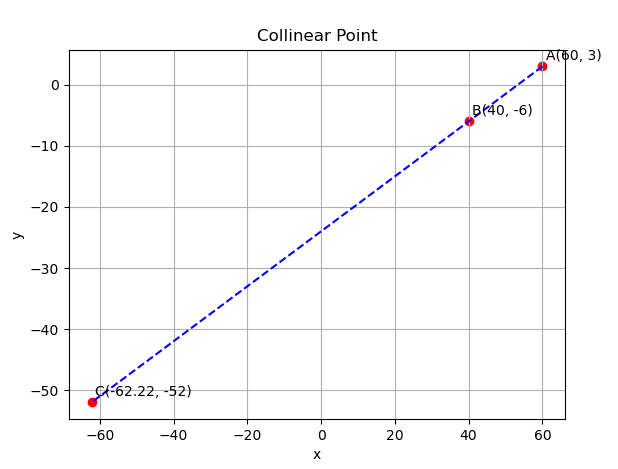
\includegraphics[width=0.6\columnwidth]{figs/fig.png}
\end{center}
\caption{}
\label{fig:Fig1}
\end{figure}
\end{document}
